\begin{figure}[t]
  \centering
  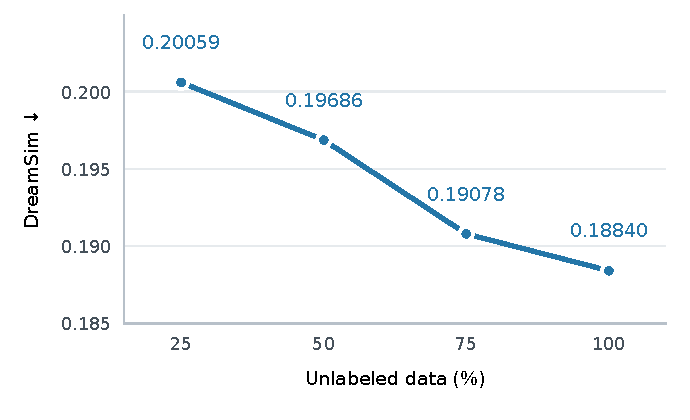
\includegraphics[width=0.68\linewidth]{figures/data_scaling/data_scaling.pdf}
  \caption{\textbf{Scaling unlabeled data on RECON.}
  The horizontal axis gives the percentage of the unlabeled data pool
  used for latent-action pretraining ($U$), with action-label availability
  fixed at $L=100\%$. After the same downstream real-action fine-tuning
  procedure, all four models are evaluated on the same 500 RECON windows
  for direct 4\,s prediction. DreamSim decreases monotonically, with a
  6.08\% relative reduction from 25\% to 100\% data. Lower is better.
  Points are single-checkpoint, single-evaluation-seed estimates;
  lines connect measurements without fitting a scaling law.}
  \label{fig:data_scaling}
\end{figure}
